\documentclass[a4paper]{article}
\addtolength{\hoffset}{-2.25cm}
\addtolength{\textwidth}{4.5cm}
\addtolength{\voffset}{-3.25cm}
\addtolength{\textheight}{5cm}
\setlength{\parindent}{15pt}

\usepackage[unicode=true, colorlinks=false, hidelinks]{hyperref}
\usepackage[utf8]{inputenc}
\usepackage[english, russian]{babel}
\usepackage{mathtext}
\usepackage[T2A, TS1]{fontenc}
\usepackage{microtype} % Slightly tweak font spacing for aesthetics
\usepackage{amsthm, amssymb, amsmath, amsfonts, nccmath}
\usepackage{nicefrac}
\usepackage{epstopdf}
\usepackage[export]{adjustbox}
\usepackage{float} % Improved interface for floating objects
\usepackage{graphicx, multicol} % Enhanced support for graphics
\usepackage{pdfrender,xcolor}
\usepackage{breqn}
\usepackage{mathtools}
\usepackage{titling}
\usepackage{bm}
\usepackage{centernot}
\usepackage[cal=boondoxo,calscaled=.96]{mathalpha}
\usepackage{marvosym, wasysym} % More symbols
\usepackage{rotating} % Rotation tools
\usepackage{censor} % Facilities for controlling restricted text

\DeclareMathOperator{\cov}{cov}
\DeclareMathOperator{\med}{med}

\usepackage{array}
\newcolumntype{C}[1]{>{\centering\let\newline\\\arraybackslash\hspace{0pt}}m{#1}}

\usepackage{fancyhdr}
\pagestyle{fancy}
\fancyhead{}\renewcommand{\headrulewidth}{0pt}
\fancyfoot[L]{}
\fancyhead{}
\fancyfoot{}
\fancyfoot[R]{\thepage}
\begin{document}
\begin{titlepage}
   \begin{center}
       \vspace*{3cm}
       \large{САНКТ-ПЕТЕРБУРГСКИЙ ПОЛИТЕХНИЧЕСКИЙ УНИВЕРСИТЕТ}
       \vspace{0.4 cm}
       
       \large\textbf{Институт прикладной математики и механики}
       \vspace{0.4 cm}
       
       \large{Высшая школа прикладной математики и вычислительной физики}
       
       \vspace{3 cm}
       \normalsize\textbf{Отчет\\ по лабораторным работам №1-4 \\ по дисциплине \\ <<Математическая статистика>>}
       \vfill
       \begin{flushright}
            \normalsize{Выполнил студент:\\
            Козлов Борис\\
            группа: 3630102/80301}
            \vskip\medskipamount
            \normalsize{Проверил:
            
            к.ф.-м.н., доцент\\
            Баженов Александр Николаевич
            }
       \end{flushright}
            
       \vspace{0.8cm}
     
            
       \normalsize{Санкт-Петербург\\2021 г.}
            
   \end{center}
\end{titlepage}
\tableofcontents
\addtocontents{toc}{~\hfill\textbf{Страница}\par}
\newpage
\listoffigures
\addtocontents{lof}{~\hfill\textbf{Страница}\par}
\newpage
\listoftables
\addtocontents{lot}{~\hfill\textbf{Страница}\par}
\newpage
\section{Постановка задачи}
\begin{enumerate}
    \item Сгенерировать двумерные выборки размерами $20,\,60,\,100$ для нормального двумерного распределения $N(x,y,0,0,1,1,\rho)$.\\
    Коэффициент корреляции $\rho$ взять равным $0,\,0.5,\,0.9$.\\
    Каждая выборка генерируется $1000$ раз и для неё вычисляются: среднее значение, среднее значение квадрата и дисперсия коэффициентов корреляции Пирсона, Спирмена и квадрантного коэффициента корреляции.\\
    Повторить все вычисления для смеси нормальных распределений:
    \begin{equation*}
        f(x,y)=0.9N(x,y,0,0,1,1,0.9)+0.1N(x,y,0,0,10,10,-0.9).
    \end{equation*}
    Изобразить сгенерированные точки на плоскости и нарисовать эллипс
    равновероятности.
    \item Найти оценки коэффициентов линейной регрессии $y_i=a+b x_i + e_i$, используя 20 точек на отрезке $[-1.8,2]$ с равномерным шагом, равным $0.2$. Ошибку $e_i$ считать нормально распределенной с параметрами $(0,1)$. В качестве эталонной зависимости взять $y_i=2+2x_i+e_i$. При построении оценок использовать 2 критерия: критерий наименьших квадратов и критерий наименьших модулей. Проделать то же самое для выборки, у которой в значения $y_1$ и $y_{20}$ вносятся возмущения $10$ и $-10$.
    \item Сгенерировать выборку объемом 100 элементов для стандартного нормального распределения. В качестве основной гипотезы $H_0$ считать, что наблюдаемая выборка принадлежит стандартному нормальному распределению. Проверить основную гипотезу, используя критерий согласия $\chi^2$. В качестве уровня значимости взять $\alpha=0.05$. Привести таблицу вычислений $\chi^2$.\\
    Исследовать точность критерия $\chi^2\;-$ сгенерировать выборки равномерного распределения и распределения Лапласа объемом 20 элементов и проверить их на нормальность.
    \item Провести дисперсионный анализ с применением критерия Фишера по данным регистраторов для одного сигнала. Определить области однородности сигнала, переходные области, фон.\\Длина сигнала равна 1024.
\end{enumerate}
\section{Теория}
\subsection{Двумерное нормальное распределение}
Двумерная случайная величина $(X, Y)$ называется распределенной нормально, если её плотность вероятности определяется формулой
\begin{align}
    N(x,y,\overline{x},\overline{y},\sigma_x,\sigma_y,\rho_{XY}^{})&=\frac{1}{2\pi\sigma_x\sigma_y\sqrt{1-\rho_{XY}^2}}\times\nonumber\\
    &\times\exp\left\{-\frac{1}{2(1-\rho_{XY}^2)}\left[\frac{\left(x-\overline{x}\right)^2}{\sigma_x^2}-2\rho_{XY}^{}\frac{(x-\overline{x})(y-\overline{y})}{\sigma_x\sigma_y}+\frac{\left(y-\overline{y}\right)^2}{\sigma_y^2}\right]\right\},
\end{align}
где $\overline{x},\,\overline{y},\sigma_x,\sigma_y$ - математические ожидания и средние квадратические отклонения компонент $X,\,Y$ соответственно, а $\rho_{XY}^{}\:-$ коэффициент корреляции. 
\subsection{Корреляционный момент и коэффициент корреляции}
\textit{Корреляционный момент} (\textit{ковариация}) двух случайных величин $X, Y$:
\begin{equation}
    K_{XY} = \cov{(X,Y)}=\mathbf{M}\left[(X-\overline{x})(Y-\overline{y})\right].
\end{equation}
\textit{Коэффициент корреляции} $\rho_{XY}$ случайных величин $X,Y$:
\begin{equation}\label{eq::rho}
    \rho_{XY}^{}=\frac{K_{XY}}{\sigma_x\sigma_y}.
\end{equation}
\textit{Ковариационной матрицей} случайного вектора $(X,Y)$ называется симметричная матрица вида
\begin{equation}
    K=\begin{pmatrix}
    D_X & K_{XY} \\
    K_{YX} & D_Y
    \end{pmatrix}.
\end{equation}
\textit{Кореляционной матрицей} случайного вектора $(X,Y)$ называется нормированная ковариационная матрица вида
\begin{equation}
    R=\begin{pmatrix}
    1 & \rho_{XY}^{} \\
    \rho_{YX}^{} & 1
    \end{pmatrix}.
\end{equation}
\subsection{Выборочные коэффициенты корреляции}
\subsubsection{Выборочный коэффициент корреляции Пирсона}
\textit{Выборочный коэффициент корреляции Пирсона}:
\begin{equation}\label{eq::pirs}
    r=\frac{\frac{1}{n}\sum_{i=1}^n \left(x_i-\overline{x}\right)\left(y_i-\overline{y}\right)}{\sqrt{\frac{1}{n}\sum_{i=1}^n\left(x_i-\overline{x}\right)^2 \frac{1}{n}\sum_{i=1}^n\left(y_i-\overline{y}\right)^2}}=\frac{K_{XY}}{s_X s_Y},
\end{equation}
где $K,\,s_X^2,\,s_Y^2\:-$ выборочные ковариация и дисперсии случайных величин $X, Y$.
\subsubsection{Выборочный коэффициент ранговой корреляции Спирмена}
Обозначим ранги, соотвествующие значениям переменной $X$, через $u$, а ранги, соответствующие значениям переменной $Y$, $-$ через $v$.
\\\\
\textit{Выборочный коэффициент ранговой корреляции Спирмена}:
\begin{equation}\label{eq::spir}
    r_S=\frac{\frac{1}{n}\sum_{i=1}^n \left(u_i-\overline{u}\right)\left(v_i-\overline{v}\right)}{\sqrt{\frac{1}{n}\sum_{i=1}^n\left(u_i-\overline{u}\right)^2 \frac{1}{n}\sum_{i=1}^n\left(v_i-\overline{v}\right)^2}},
\end{equation}
где $\overline{u}=\overline{v}=\frac{1+2+...+n}{n}=\frac{n+1}{2}\,-$ среднее значение рангов.
\subsubsection{Выборочный квадрантный коэффициент корреляции}
\begin{equation}\label{eq::rQ}
    r_Q=\frac{(n_1+n_3)-(n_2+n_4)}{n},
\end{equation}
где $n_1,n_2,n_3,n_4\:-$ количества точек с координатами $(x_i,y_i)$, попавшими соответственно в I, II, III и IV квадранты декартовой системы с осями $x^'=x-\med{x},\,y^'=y-\med{y}$ и с центром в точке с координатами $(\med{x},\med{y})$.
\subsection{Эллипсы рассеивания}
Уравнение проекции эллипса рассеивания на плоскость $xOy$:
\begin{equation}\label{eq:ellipse}
    \frac{\left(x-\overline{x}\right)^2}{\sigma_x^2}-2\rho_{XY}^{}\frac{(x-\overline{x})(y-\overline{y})}{\sigma_x\sigma_y}+\frac{\left(y-\overline{y}\right)^2}{\sigma_y^2}=C,\;\;C\,-\,\text{const}.
\end{equation}
Центр эллипса \eqref{eq:ellipse} находится в точке с координатами $(\overline{x},\overline{y})$, оси симметрии эллипса составляют с осью $Ox$ углы, определяемые уравнением
\begin{equation}
    \tan{2\alpha}=\frac{2\rho_{XY}^{}\sigma_x\sigma_y}{\sigma_x^2-\sigma_y^2}.
\end{equation}
\subsection{Простая линейная регрессия}
\subsubsection{Модель простой линейной регрессии}
Регрессионую модель описания данных называют \textit{простой линейной регрессией}, если
\begin{equation}
    y_i=\beta_0 + \beta_1 x_i + \varepsilon_i,\;\;i=1,...,n,
\end{equation}
где $x_1, ..., x_n\:-$ заданные числа (значения фактора); $y_1,...,y_n\:-$ наблюдаемые значения отклика; $\varepsilon_1,...,\varepsilon_n\:-$ независимые, нормально распределенные $N(0,\sigma)$ с нулевым математическим ожиданием и одинаковой (неизвестной) дисперсией случайные величины (ненаблюдаемые); $\beta_0,\:\beta_1\:-$ неизвестные параметры, подлежащие оцениванию.
\subsubsection{Метод наименьших квадратов}
\textit{Метод наименьших квадратов} (МНК):
\begin{equation}
    Q\left(\beta_0,\beta_1\right)=\sum_{i=1}^n \varepsilon_i^2= \sum_{i=1}^n\left(y_i-\beta_0-\beta_1 x_i\right)^2\to\min_{\beta_0,\beta_1}.
\end{equation}
\subsubsection{Расчётные формулы для МНК-оценок}
МНК-оценки параметров $\beta_0$ и $\beta_1$:
\begin{equation}
    \widehat{\beta}_1=\frac{\overline{xy}-\overline{x}\cdot\overline{y}}{\overline{x^2}-(\overline{x})^2},
\end{equation}
\begin{equation}
    \widehat{\beta}_0=\overline{y}-\overline{x}\widehat{\beta}_1.
\end{equation}
\subsection{Робастные оценки коэффициентов линейной регрессии}
\textit{Метод наименьших модулей}:
\begin{equation}
    \sum_{i=1}^n |y_i-\beta_0-\beta_1 x_i|\to \min_{\beta_0,\beta_1}.
\end{equation}
\begin{equation}
    \widehat{\beta}_{1R}=r_Q\frac{q_y^*}{q_x^*},
\end{equation}
\begin{equation}
    \widehat{\beta}_{0R}=\med{y}-\widehat{\beta}_{1R}\med{x},
\end{equation}
\begin{equation}
    r_Q=\frac{1}{n}\sum_{i=1}^n \sign{(x_i-\med{x})}\sign{(y_i-\med{y})},
\end{equation}
\begin{equation}
    q_y^*=\frac{y_{(j)}-y_{(l)}}{k_q(n)},\;\;q_x^*=\frac{x_{(j)}-x_{(l)}}{k_q(n)},
\end{equation}
\begin{equation*}
    k_q(20)=1.491.
\end{equation*}
\begin{equation*}
    \sign{z} = [z>0] - [z<0],\;\;[\,.\,]-\text{скобка Айверсона},
\end{equation*}
\begin{equation*}
    l = \lfloor n/4 \rfloor + \left[\,n/4 \not\in \mathbb{Z}\,\right],
\end{equation*}
\begin{equation*}
    j=n-l+1.
\end{equation*}
Уравнение регрессии здесь имеет вид
\begin{equation}
    y = \widehat{\beta}_{0R}+\widehat{\beta}_{1R} x.
\end{equation}
\subsection{Проверка гипотезы о законе распределения генеральной совокупности. Метод хи-квадрат}
Выдвинута гипотеза $H_0$ о генеральном законе распределения с функцией
распределения $F(x)$.\\
Рассматриваем случай, когда гипотетическая функция распределения $F(x)$ не содержит неизвестных параметров.\\
Для вычисления $k$ будем руководствоваться формулой
\begin{equation*}
    k\approx 1.72\sqrt[3]{n}.
\end{equation*}
\subsubsection*{Правило проверки гипотезы о законе распределения по методу $\chi^2$}
\begin{enumerate}
    \item Выбираем уровень значимости $\alpha$.
    \item По таблице \cite[с. 572-573]{book1} находим квантиль $\chi_{1-\alpha}^2(k-1)$ распределения хи-квадрат с $k-1$ степенями свободы порядка $1-\alpha$.
    \item Вычисляем вероятности $p_i=P(X\in\Delta_i), i = 1,...,k$, с помощью гипотетической функции распределения $F(x)$.
    \item Находим частоты $n_i$ попадания элементов выборки в подмножества $\Delta_i,i=1,...,k$.
    \item Вычисляем выборочное значение статистики критерия $\chi^2$:
        \begin{equation*}
            \chi^2_{\text{В}}=\sum_{i=1}^k\frac{(n_i-np_i)^2}{np_i}.
        \end{equation*}
    \item Сравниваем $\chi^2_{\text{В}}$ и квантиль $\chi_{1-\alpha}^2(k-1)$.
        \begin{enumerate}
            \item Если $\chi^2_{\text{В}}<\chi_{1-\alpha}^2(k-1)$, то гипотеза $H_0$ на данном этапе проверки принимается.
            \item Если $\chi^2_{\text{В}}\geq\chi_{1-\alpha}^2(k-1)$, то гипотеза $H_0$ отвергается, выбирается одно из альтернативных распределений, и процедура проверки повторяется.

        \end{enumerate}
\end{enumerate}
\subsection{Дисперсионный анализ с применением критерия Фишера}
Пусть дана выборка
\begin{equation*}
    X = \{x_1,\hdots, x_n\},
\end{equation*}
разделенная на $k$ подвыборок вида
\begin{equation*}
    X_1 = \{x_{11},\hdots, x_{1n_1}\},
\end{equation*}
\begin{equation*}
    \hdots
\end{equation*}
\begin{equation*}
    X_k = \{x_{k1},\hdots, x_{kn_k}\}.
\end{equation*}
\begin{equation*}
    X=\bigcup_{1\leq i\leq k} X_i,
\end{equation*}
\begin{equation*}
    i\neq j\Longrightarrow X_i \cap X_j = \varnothing.
\end{equation*}
Пусть $s_i^2$ и $\overline{X}_i\;-$ дисперсия и среднее подвыборки $X_i$. Величина
\begin{equation*}
    \overline{X}=\dfrac{1}{k}\sum_{i=1}^k \overline{X}_i
\end{equation*}
называется средней общей. Внутригрупповой дисперсией называется величина вида
\begin{equation}
    \widehat{\sigma}^2=\dfrac{1}{k}\sum_{i=1}^k s_i^2,
\end{equation}
а межгрупповой $-$
\begin{equation}
    \delta^2=\dfrac{1}{n}\sum_{i=1}^k\left(\overline{X}_i-\overline{X}\right)^2  n_i.
\end{equation}
Критерием Фишера $F$ называется следующее отношение:
\begin{equation}
    F=\dfrac{\delta^2}{\widehat{\sigma}^2}.
\end{equation}
\subsubsection*{Этапы разведочного анализа}
\begin{itemize}
    \item Извелечение сигнала из входных данных.
    \item Построение и анализ гистограммы сигнала. Значения в столбце с наибольшей высотой отвечают за фон, значения в столбце со второй по величине высотой отвечают за сигнал, все остальные значения отвечают за переходы.
    \item Фильтрация сигнала медианным фильтром с размером окна, равным 3.
\end{itemize}
Далее однородность каждого промежутка оценивается с помощью критерия Фишера.
\section{Реализация}
Лабораторная работа выполнена на языке R в средe R Studio с использованием следующих библиотек:
\begin{enumerate}
        \item MASS (генерация выборок)
        \item kableExtra (оформление)
        \item ggplot2, cowplot (визуализация данных)
\end{enumerate}
\section{Результаты}
\subsection{Выборочные коэффициенты корреляции}
\begin{table}[H]
    \centering
    \begin{tabular}{|l|c|c|c|}
    \hline 
    $\rho = 0.0$&$r$\eqref{eq::pirs}&$r_s$\eqref{eq::spir}&$r_Q$\eqref{eq::rQ}\\\hline 
$E(z)$&0.006&0.009&0.009\\\hline 
$E(z^2)$&0.052&0.051&0.051\\\hline 
$D(z)$&0.052&0.051&0.051\\\hline 

    \end{tabular}\\
    \begin{center}
        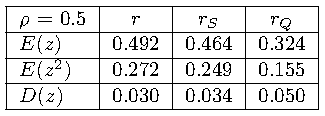
\includegraphics[]{LabSrcs/resources/20rho0.5.pdf}
    \end{center}
    \begin{center}
        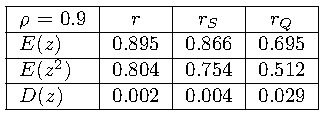
\includegraphics{LabSrcs/resources/20rho0.9.pdf}
    \end{center}
    \caption{Двумерное нормальное распределение, $n=20$}
    \label{tab:norm20}
\end{table}
\begin{table}[H]
    \begin{center}
    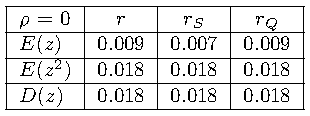
\includegraphics[]{LabSrcs/resources/60rho0.pdf}
    \end{center}
    \begin{center}
    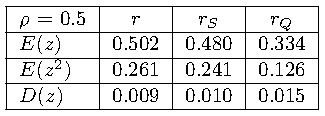
\includegraphics[]{LabSrcs/resources/60rho0.5.pdf}
    \end{center}
    \begin{center}
    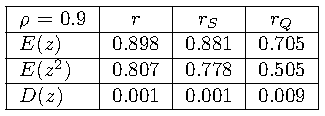
\includegraphics[]{LabSrcs/resources/60rho0.9.pdf}
    \end{center}
    \caption{Двумерное нормальное распределение, $n=60$}
    \label{tab:norm60}
\end{table}
\begin{table}[H]
    \begin{center}
    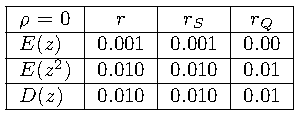
\includegraphics[]{LabSrcs/resources/100rho0.pdf}
    \end{center}
    \begin{center}
    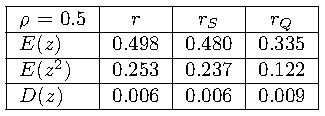
\includegraphics[]{LabSrcs/resources/100rho0.5.pdf}
    \end{center}
    \begin{center}
    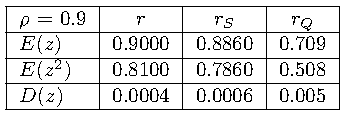
\includegraphics[]{LabSrcs/resources/100rho0.9.pdf}
    \end{center}
    \caption{Двумерное нормальное распределение, $n=100$}
    \label{tab:norm100}
\end{table}
\begin{table}[H]
    \begin{center}
    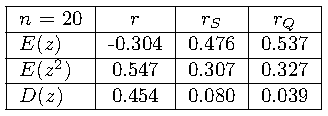
\includegraphics[]{LabSrcs/resources/mixedDistr20.pdf}
    \end{center}
    \begin{center}
    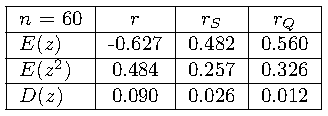
\includegraphics[]{LabSrcs/resources/mixedDistr60.pdf}
    \end{center}
    \begin{center}
    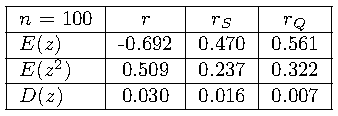
\includegraphics[]{LabSrcs/resources/mixedDistr100.pdf}
    \end{center}
    \caption{Смесь нормальных распределений}
    \label{tab:mixture}
\end{table}
\subsection{Эллипсы рассеивания}
Положим $C=k^2$. Так как $\sigma_x=\sigma_y=1,\;\overline{x}=\overline{y}=0$, то во всех 3 случаях уравнение эллипса будет иметь вид
\begin{equation*}
    E:x^2-2\rho xy + y^2=k^2,
\end{equation*}
а функция плотности вероятности $-$
\begin{equation*}
    f(x,y)=\dfrac{1}{2\pi\sqrt{1-\rho^2}}\cdot e^{-\frac{1}{2(1-\rho^2)}(x^2-2\rho xy + y^2)}.
\end{equation*}
Тогда
\begin{equation*}
 \mathbf{P}\left((X,Y)\subset E\right)=\iint \limits_{E}f(x,y) dx dy.
\end{equation*}
Обозначим интеграл за $I$. Произведем замену
\begin{equation*}
    \begin{cases}
    x=\frac{x_1}{\sqrt{2}}+\frac{y_1}{\sqrt{2}},\\
    y=-\frac{x_1}{\sqrt{2}}+\frac{y_1}{\sqrt{2}}.
    \end{cases}
\end{equation*}
Якобиан такого отображения равен 1.\\
$E$ в данном случае примет вид
\begin{equation*}
    E_1:(1+\rho)x_1^2+(1-\rho)y_1^2=k^2.
\end{equation*}
Интеграл равен
\begin{equation*}
    I=\dfrac{1}{2\pi\sqrt{1-\rho^2}}\iint \limits_{E_1}e^{-\frac{1}{2(1-\rho^2)}((1+\rho)x_1^2+(1-\rho)y_1^2)}dx_1 dy_1.
\end{equation*}
Повторно произведем замену
\begin{equation*}
    \begin{cases}
    x_1=\dfrac{u}{\sqrt{1+\rho}},\\
    y_1=\dfrac{v}{\sqrt{1-\rho}}.
    \end{cases}
\end{equation*}
Якобиан данного отображения равен $\dfrac{1}{\sqrt{1-\rho^2}}$.\\
$E_1$ принимает вид
\begin{equation*}
    R: u^2+v^2=k^2.
\end{equation*}
Интеграл равен
\begin{equation*}
    I=\dfrac{1}{2\pi(1-\rho^2)}\iint \limits_{R}e^{-\frac{1}{2(1-\rho^2)}(u^2+v^2)}du dv.
\end{equation*}
Переход к полярной системе координат:
\begin{equation*}
    \begin{cases}
    u=r\sin{\varphi},\\
    v=r\cos{\varphi}.
    \end{cases}
\end{equation*}
Якобиан преобразования равен $r$.\\
\begin{equation*}
    I=\dfrac{1}{2\pi(1-\rho^2)}\int\limits_{0}^{2\pi}d\varphi\int\limits_{0}^{k}r e^{-\frac{r^2}{2(1-\rho^2)}}dr=1-\exp\left\{-\dfrac{k^2}{2(1-\rho^2)}\right\}.
\end{equation*}
Определим $C$ для $95\%$-процентной доверительной области:
\begin{equation*}
    0.95=1-\exp\left\{-\dfrac{k^2}{2(1-\rho^2)}\right\}\Longrightarrow \exp\left\{-\dfrac{k^2}{2(1-\rho^2)}\right\}=0.05\Longrightarrow -\dfrac{k^2}{2(1-\rho^2)}=\ln{0.05},
\end{equation*}
\begin{equation*}
    C=k^2=2(\rho^2-1)\ln{0.05}\,.
\end{equation*}
Тогда
\begin{equation*}
    \text{Для }\rho=0:C=-2\ln{0.05}\approx6,
\end{equation*}
\begin{equation*}
    \text{Для }\rho=0.5:C=-2\ln{0.05}\approx4.5,
\end{equation*}
\begin{equation*}
    \text{Для }\rho=0.9:C=-2\ln{0.05}\approx1.14,
\end{equation*}
\begin{figure}[H]
    \centering
    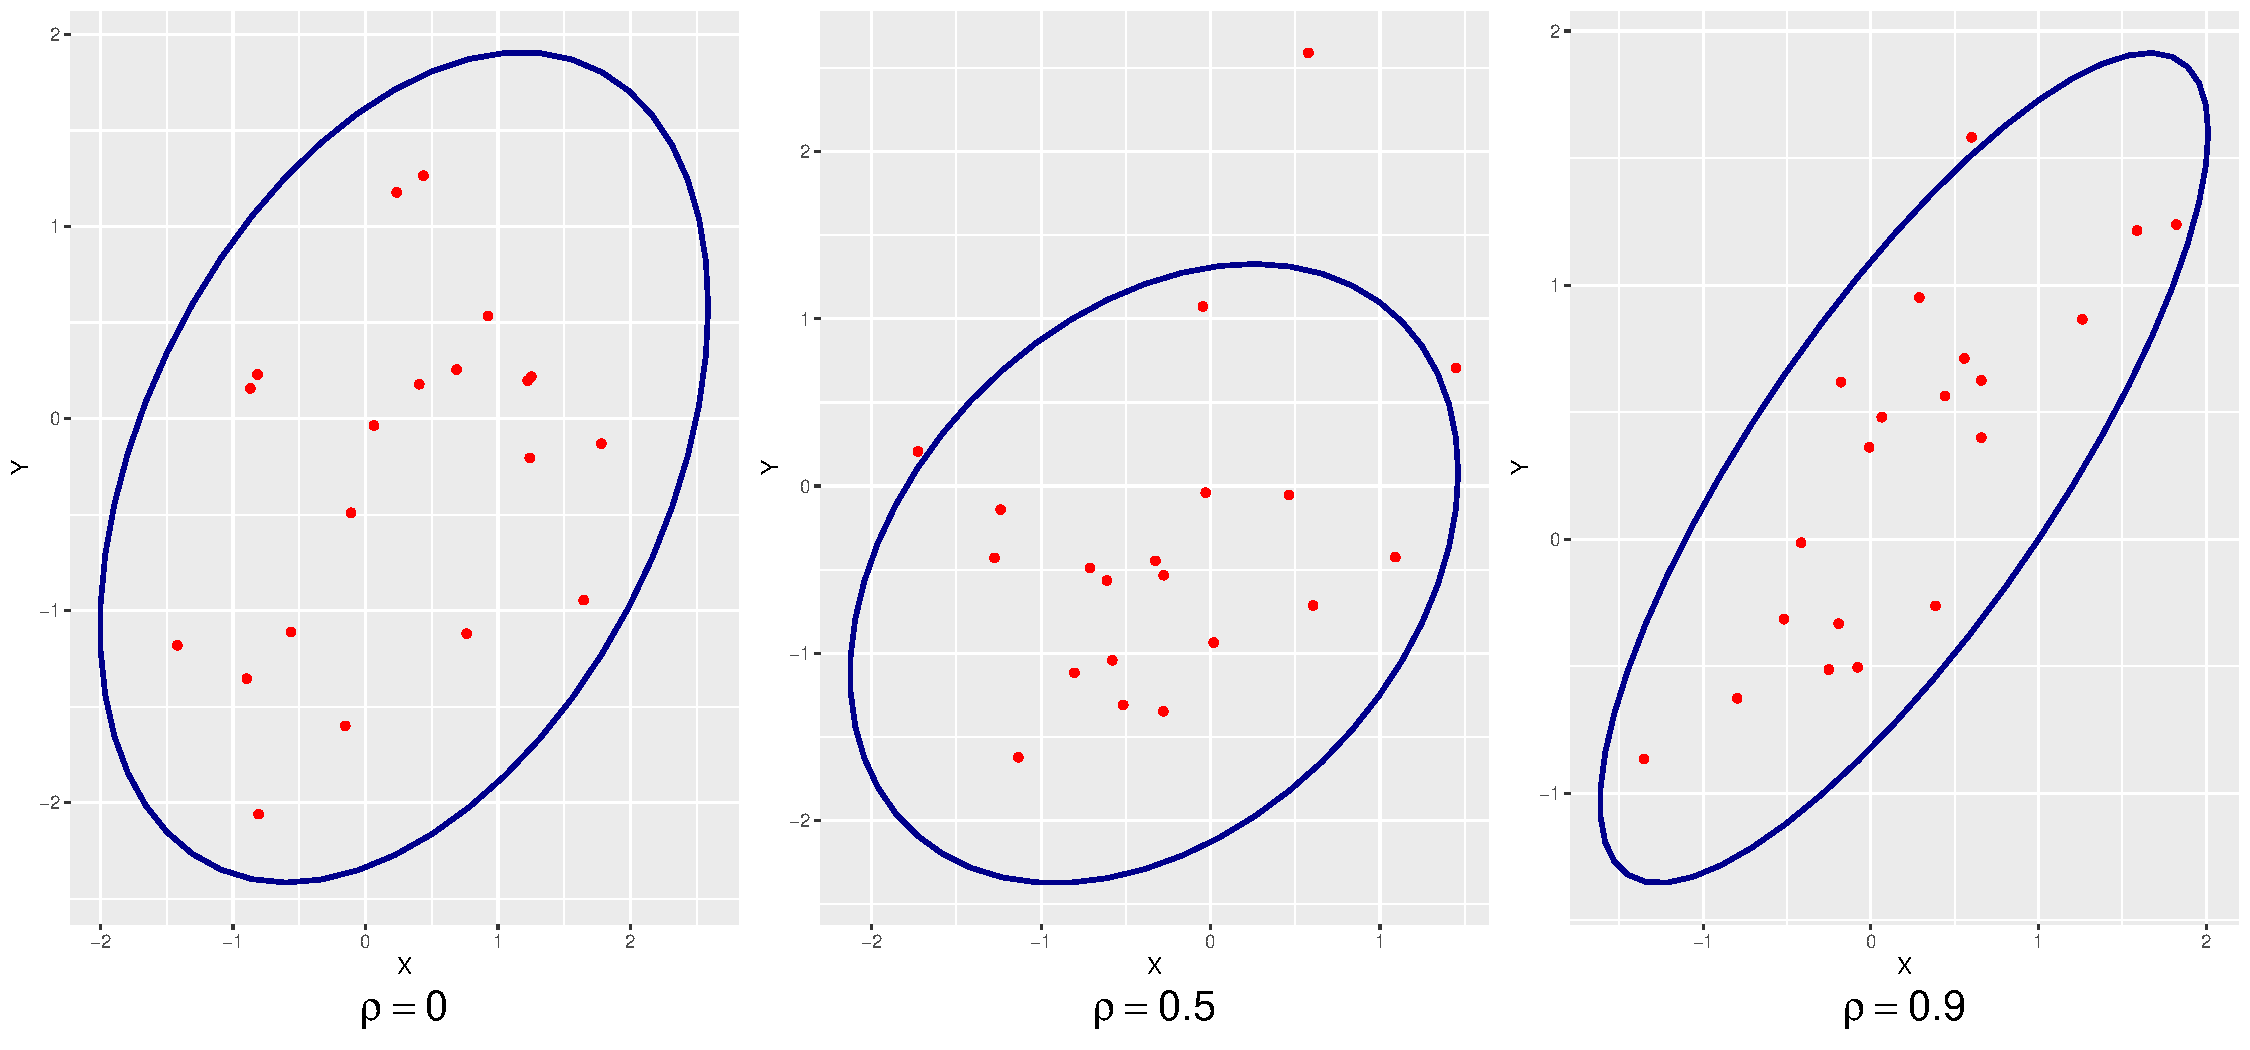
\includegraphics[width = \textwidth, height = 7 cm]{LabSrcs/resources/ellipse20.pdf}
    \caption{Двумерное нормальное распределение, $n=20$}
    \label{fig:el20}
\end{figure}
\begin{figure}[H]
    \centering
    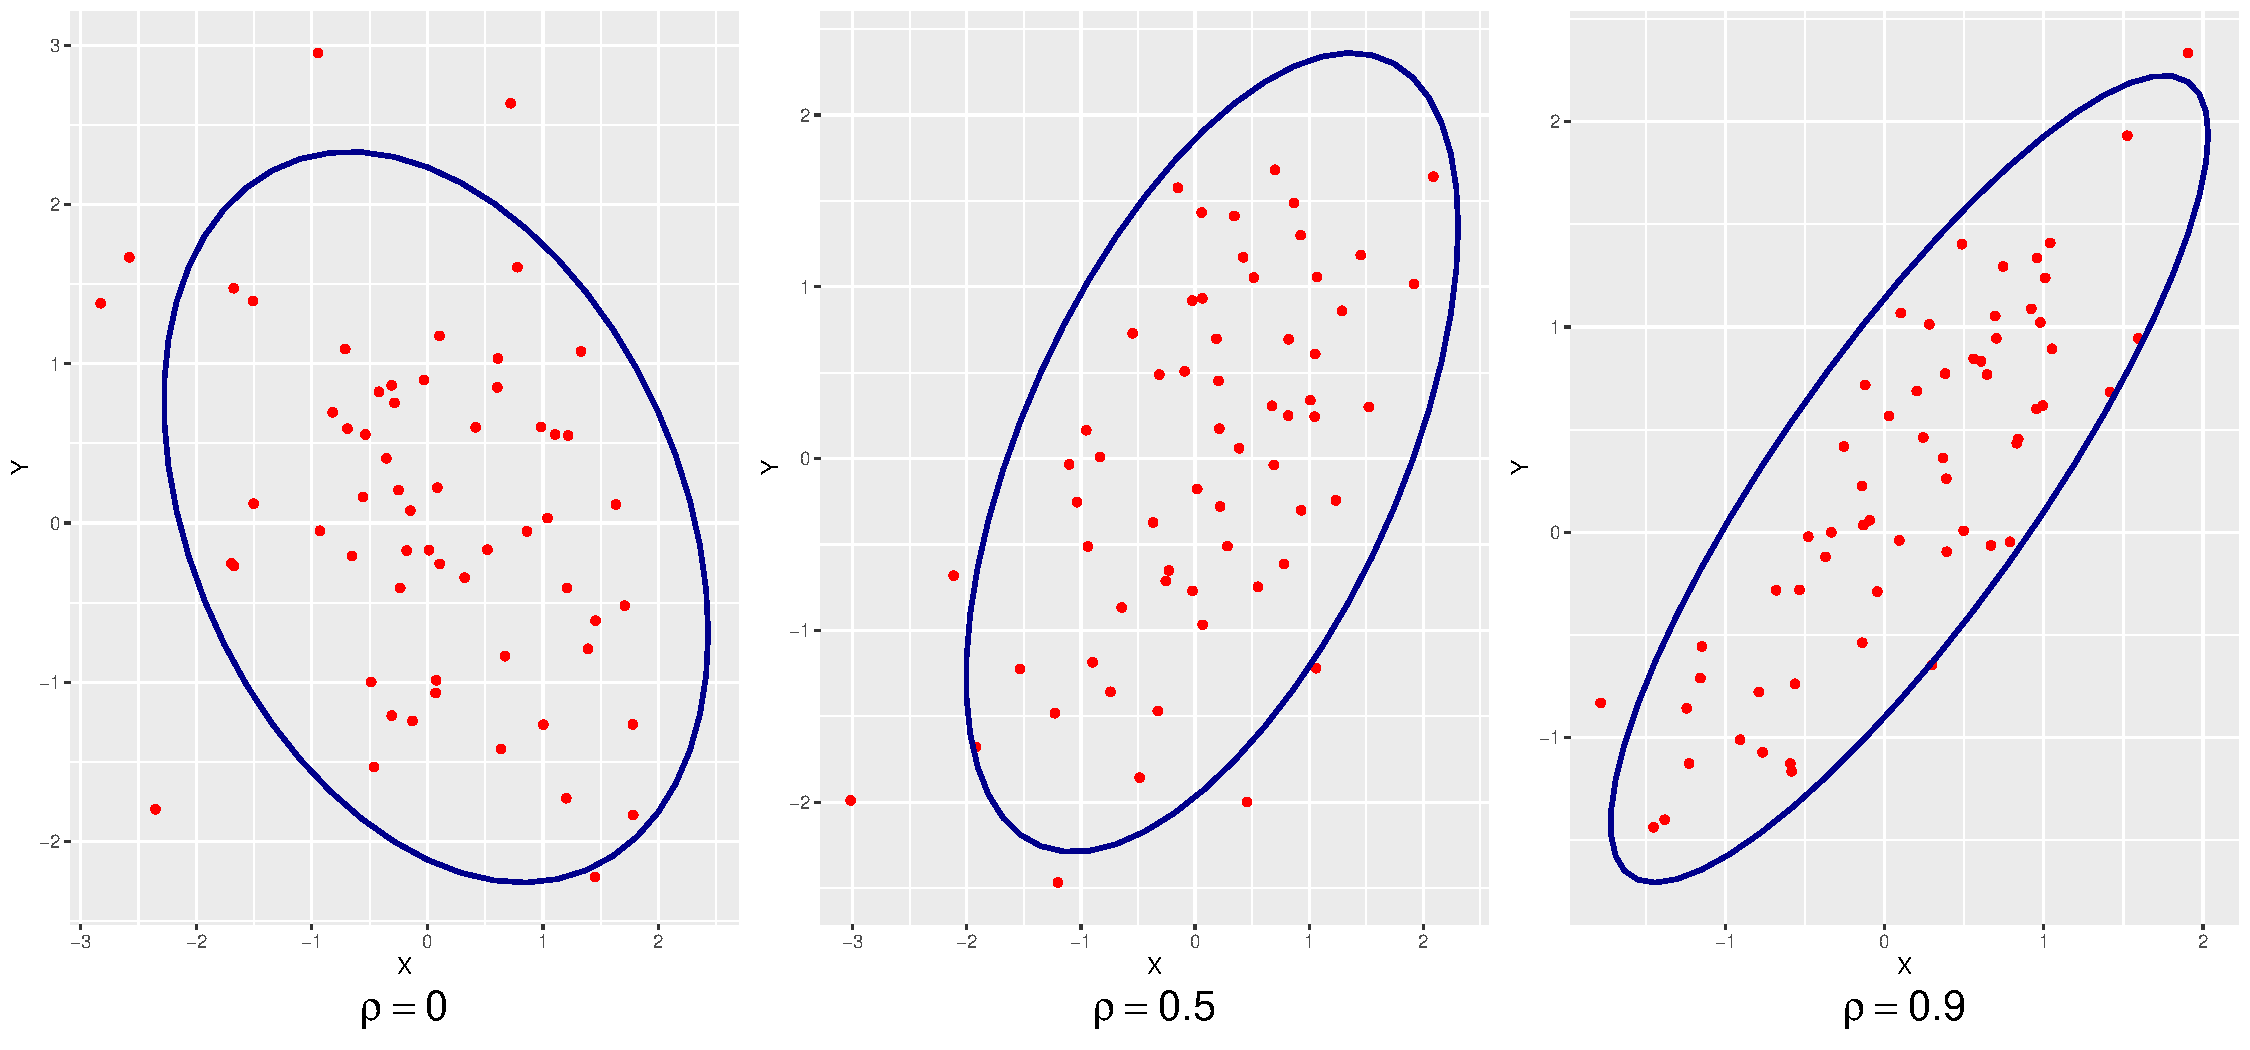
\includegraphics[width = \textwidth, height = 7 cm]{LabSrcs/resources/ellipse60.pdf}
    \caption{Двумерное нормальное распределение, $n=60$}
    \label{fig:el60}
\end{figure}
\begin{figure}[H]
    \centering
    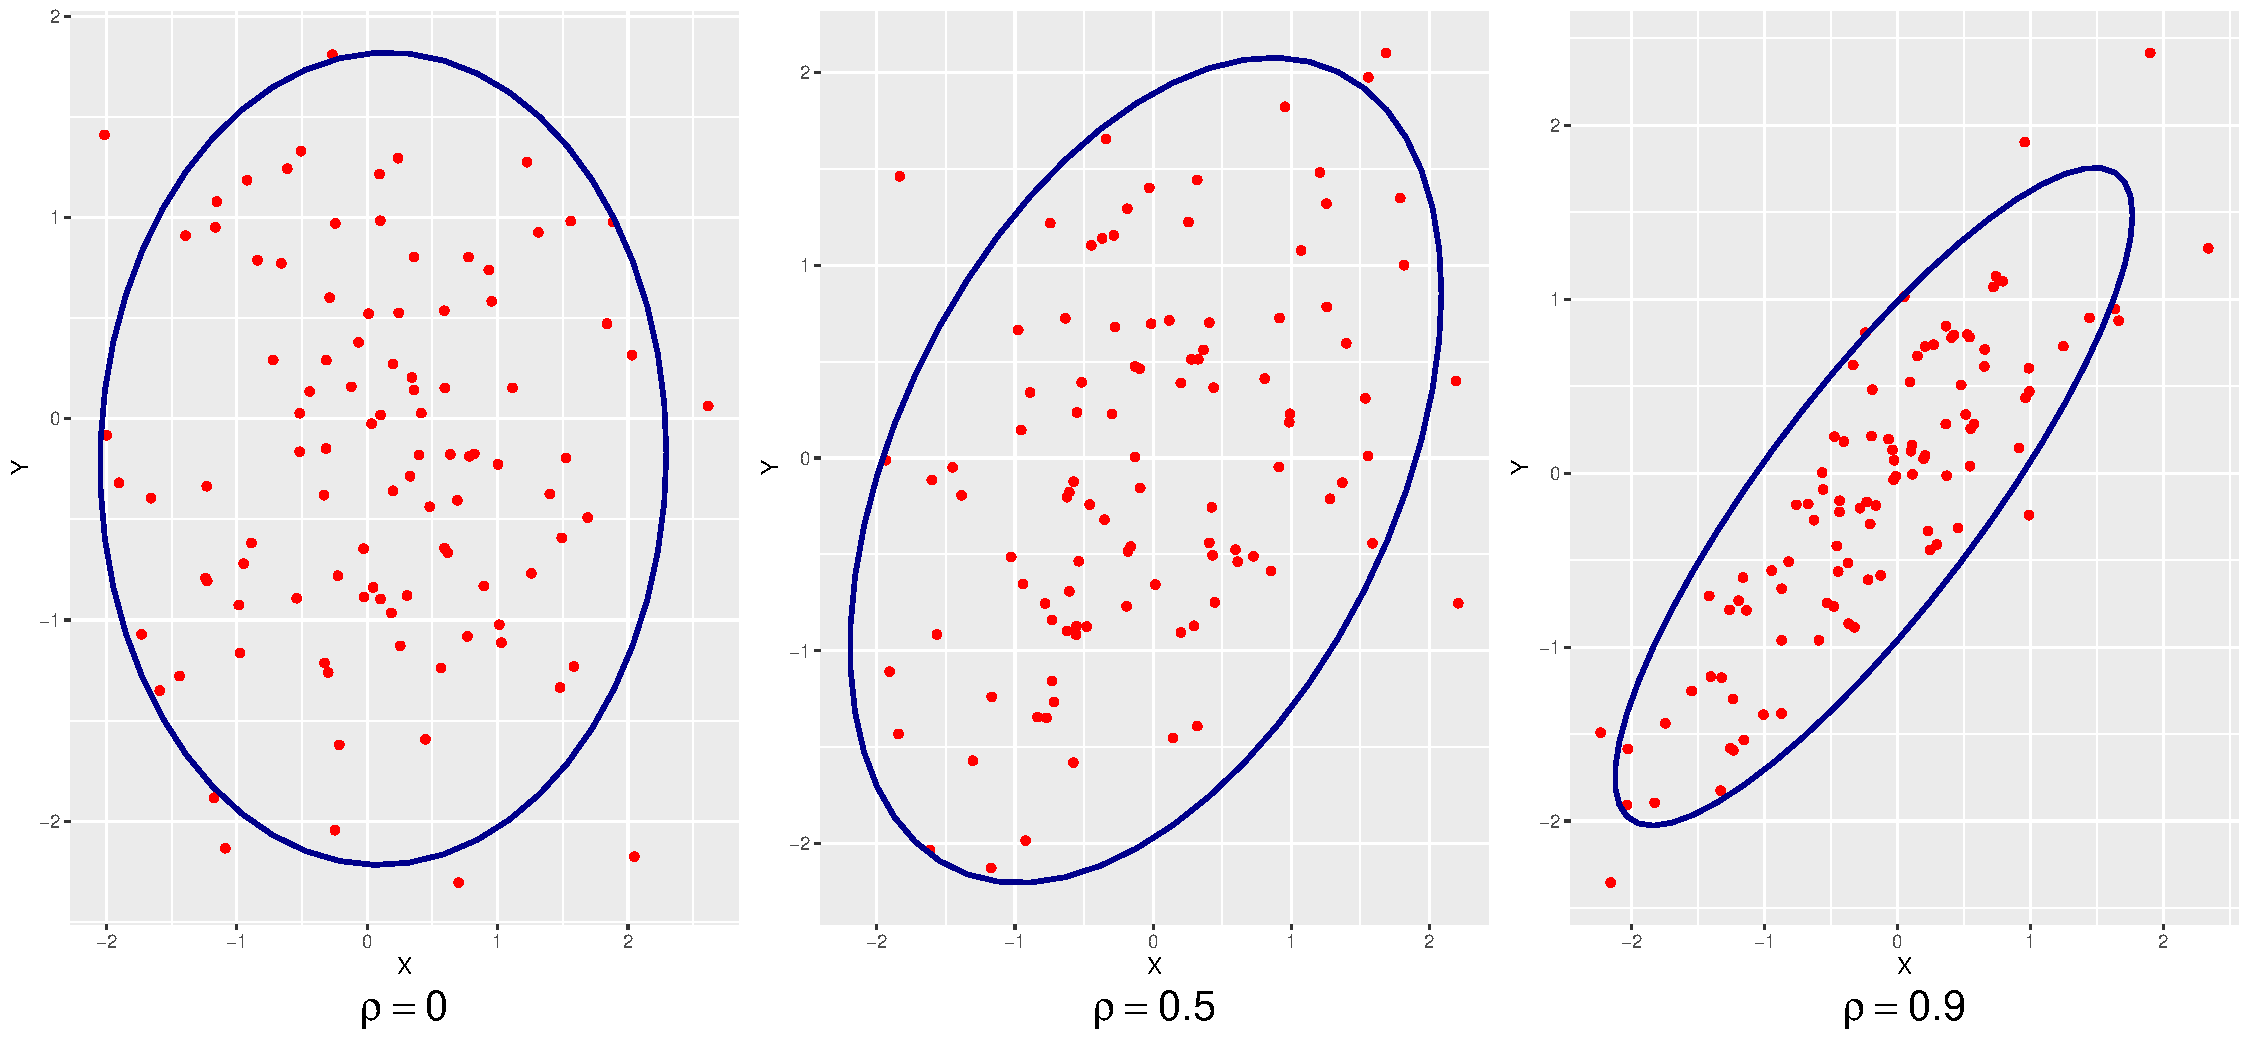
\includegraphics[width = \textwidth, height = 7 cm]{LabSrcs/resources/ellipse100.pdf}
    \caption{Двумерное нормальное распределение, $n=100$}
    \label{fig:el100}
\end{figure}
\subsection{Оценки коэффициентов линейной регрессии}
\subsubsection{Выборка без возмущения}
\begin{itemize}
    \item Критерий наименьших квадратов (LS):
    \[
    \beta_0 \approx 1.81\;\;\beta_1 \approx 1.89
.
    \]
    \item Критерий наименьших модулей (LAD):
    \[
    \beta_{0R} \approx 2.09\;\;\beta_{1R} \approx 1.5
.
    \]
\end{itemize}
\begin{figure}[H]
    \centering
    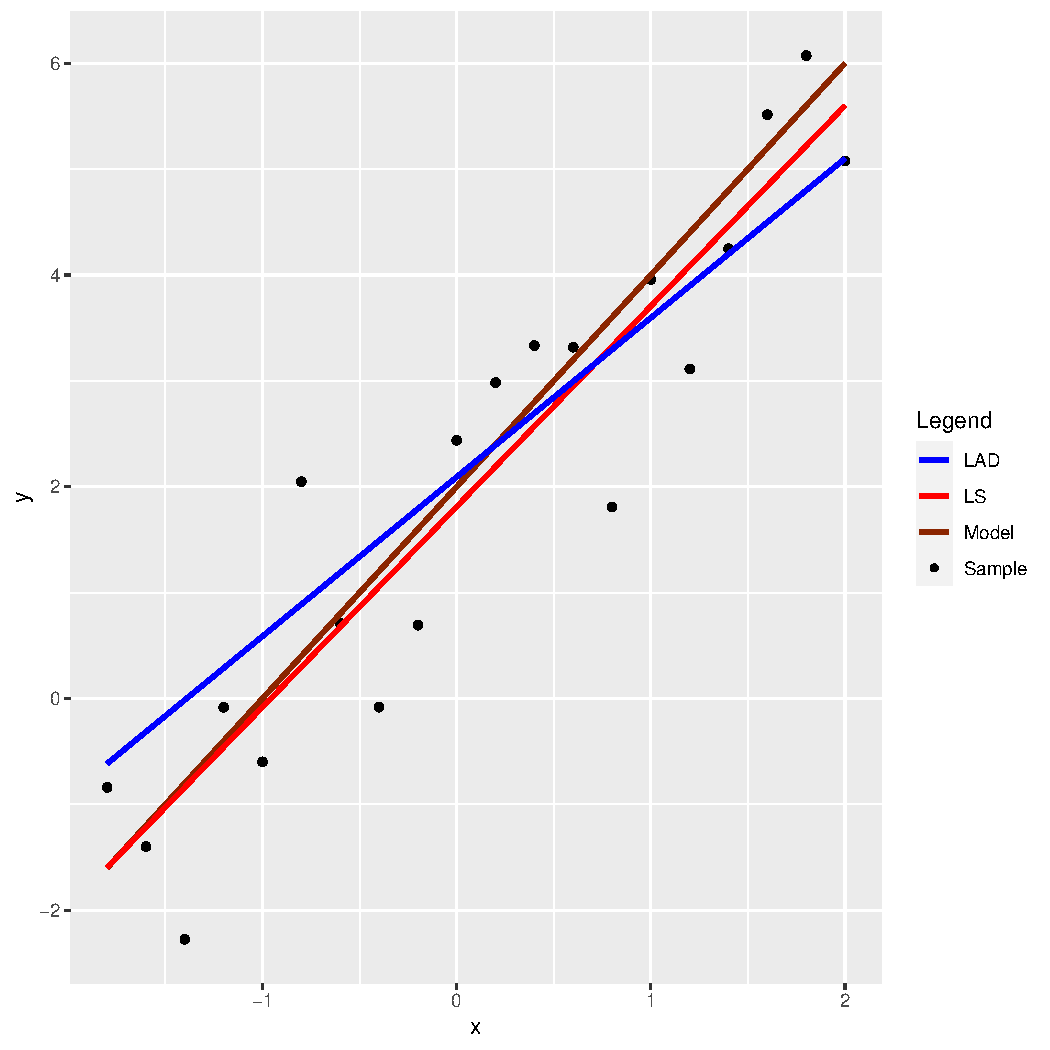
\includegraphics[width = 12 cm ]{LabSrcs/resources/usual_sample_regression.pdf}
    \caption{Выборка без возмущений}
    \label{fig:usr}
\end{figure}
\subsubsection{Выборка с возмущениями}
\begin{itemize}
    \item Критерий наименьших квадратов:
    \[
    \beta_0 \approx 1.95\;\;\beta_1 \approx 0.41
.
    \]
    \item Критерий наименьших модулей:
    \[
    \beta_{0R} \approx 2.01\;\;\beta_{1R} \approx 1.68
.
    \]
\end{itemize}
\begin{figure}[H]
    \centering
    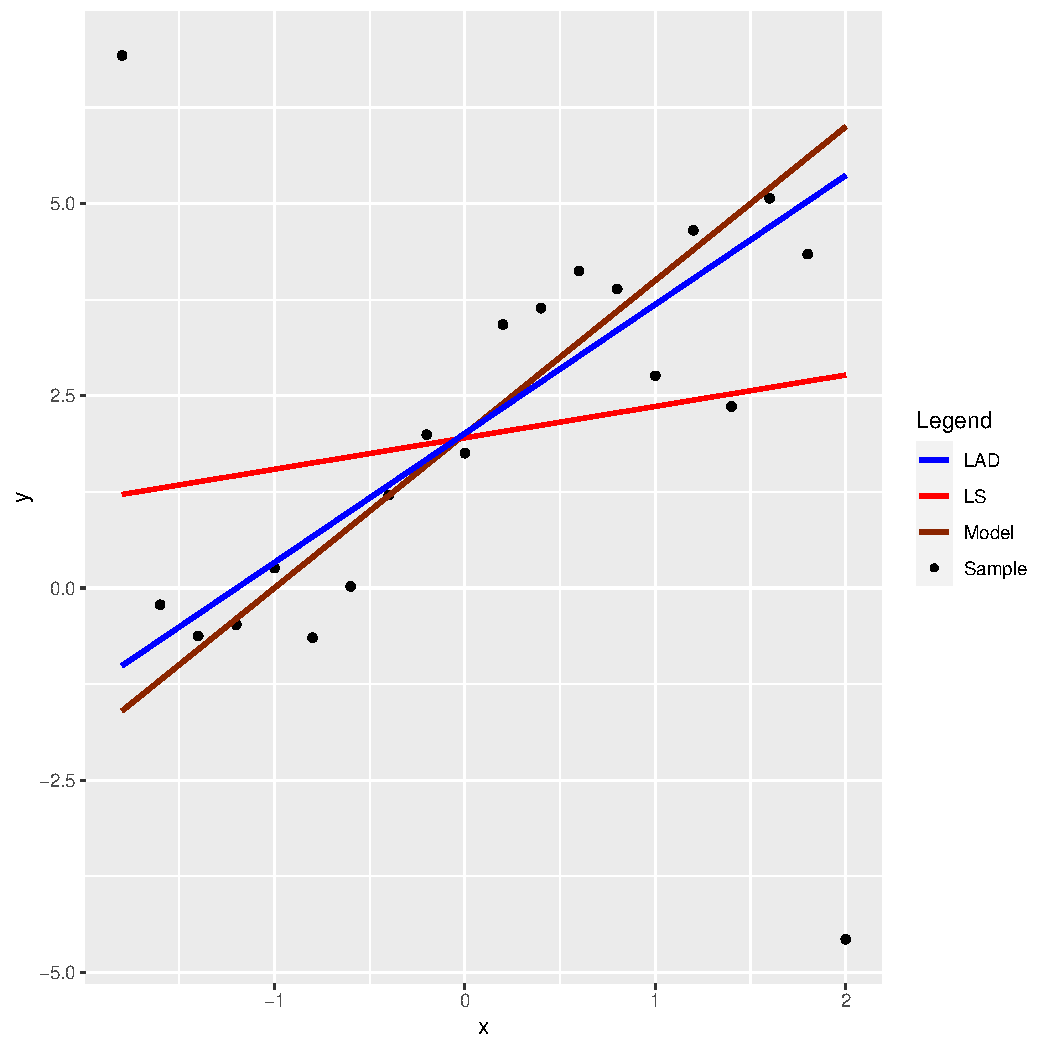
\includegraphics[width = 12 cm ]{LabSrcs/resources/perturbated_sample_regression.pdf}
    \caption{Выборка c возмущениями}
    \label{fig:perr}
\end{figure}
\subsection{Проверка гипотезы о законе распределения генеральной совокупности. Метод хи-квадрат}
\begin{itemize}
    \item Количество промежутков $k=1.72\sqrt[3]{100}=7.984\approx8$,
    \item Уровень значимости $\alpha=0.05$,
    \item Квантиль из таблицы $\chi^2_{0.95}(7)\approx 14.1$.
\end{itemize}
\begin{table}[H]
    \centering
    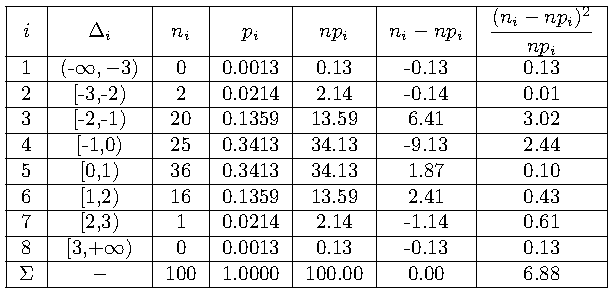
\includegraphics[]{LabSrcs/resources/chi2test.pdf}
    \caption{$\chi^2$-тест для $N(0,1)$.}
    \label{tab:chi2test}
\end{table}
\begin{equation*}
    6.92=\chi_{\text{В}}^2<\chi_{0.95}^2(7)\;\Longrightarrow\;H_0\text{ принимается}
.
\end{equation*}
\subsection*{Исследование на чувствительность}
\begin{enumerate}
    \item Рассмотрим гипотезу $H_0$ о нормальности выборки, сгенерированной согласно распределению Лапласа $L(0,\frac{1}{\sqrt{2}})$. Используем критерий согласия $\chi^2$:
    \begin{itemize}
    \item Количество промежутков $k=1.72\sqrt[3]{20}\approx5$,
    \item Уровень значимости $\alpha=0.05$,
    \item Квантиль из таблицы $\chi^2_{0.95}(4)\approx 9.5$.
\end{itemize}
\begin{table}[H]
    \centering
    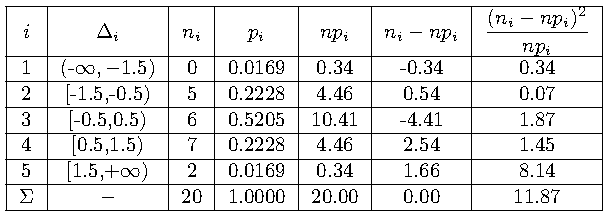
\includegraphics[]{LabSrcs/resources/chi2testLaplace.pdf}
    \caption{тест на нормальность выборки по Лапласу.}
    \label{tab:chi2lapl}
\end{table}
\begin{equation*}
    10.41=\chi_{\text{В}}^2\not<\chi_{0.95}^2(4)\;\Longrightarrow\;$H_0$\text{ на данном этапе не принимается}
.
\end{equation*}
\item Рассмотрим гипотезу $H_0$ о нормальности выборки, сгенерированной согласно равномерному распределению $U(-1.5,1.5)$. Используем критерий согласия $\chi^2$:
    \begin{itemize}
    \item Количество промежутков $k=1.72\sqrt[3]{20}\approx5$,
    \item Уровень значимости $\alpha=0.05$,
    \item Квантиль из таблицы $\chi^2_{0.95}(4)\approx 9.5$.
\end{itemize}
\begin{table}[H]
    \centering
    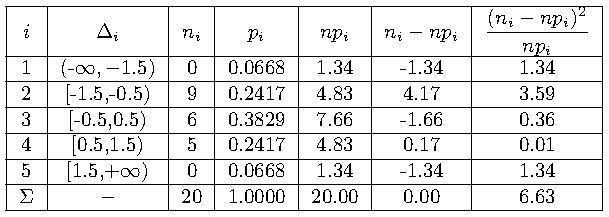
\includegraphics[]{LabSrcs/resources/chi2testUnif.pdf}
    \caption{Тест на нормальность выборки, подчиняющейся равномерному распределению.}
    \label{tab:chi2unif}
\end{table}
\begin{equation*}
    8.98=\chi_{\text{В}}^2<\chi_{0.95}^2(4)\;\Longrightarrow\;\$H_0$\text{ принимается}
.
\end{equation*}
\end{enumerate}
\subsection{Дисперсионный анализ с применением критерия Фишера}
В работе рассматривался сигнал с индексом 75.
\begin{figure}[H]
    \centering
    \begin{minipage}{0.5\textwidth}
        \centering
        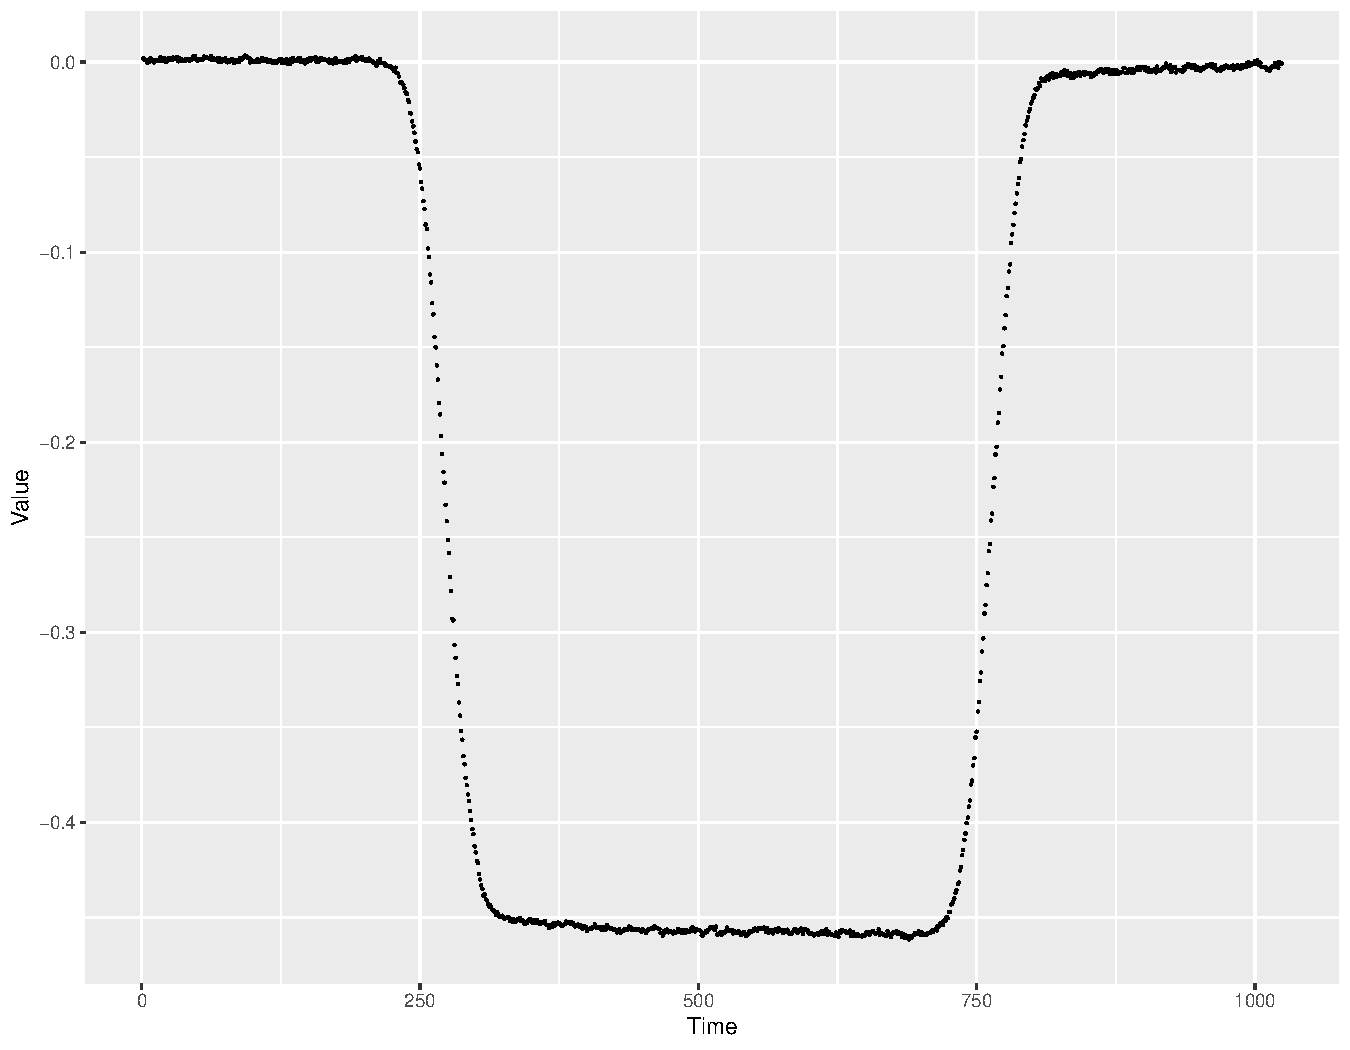
\includegraphics[width=\textwidth]{LabSrcs/resources/wave_pic.pdf}
        \caption{Входной сигнал}
    \end{minipage}\hfill
    \begin{minipage}{0.5\textwidth}
        \centering
        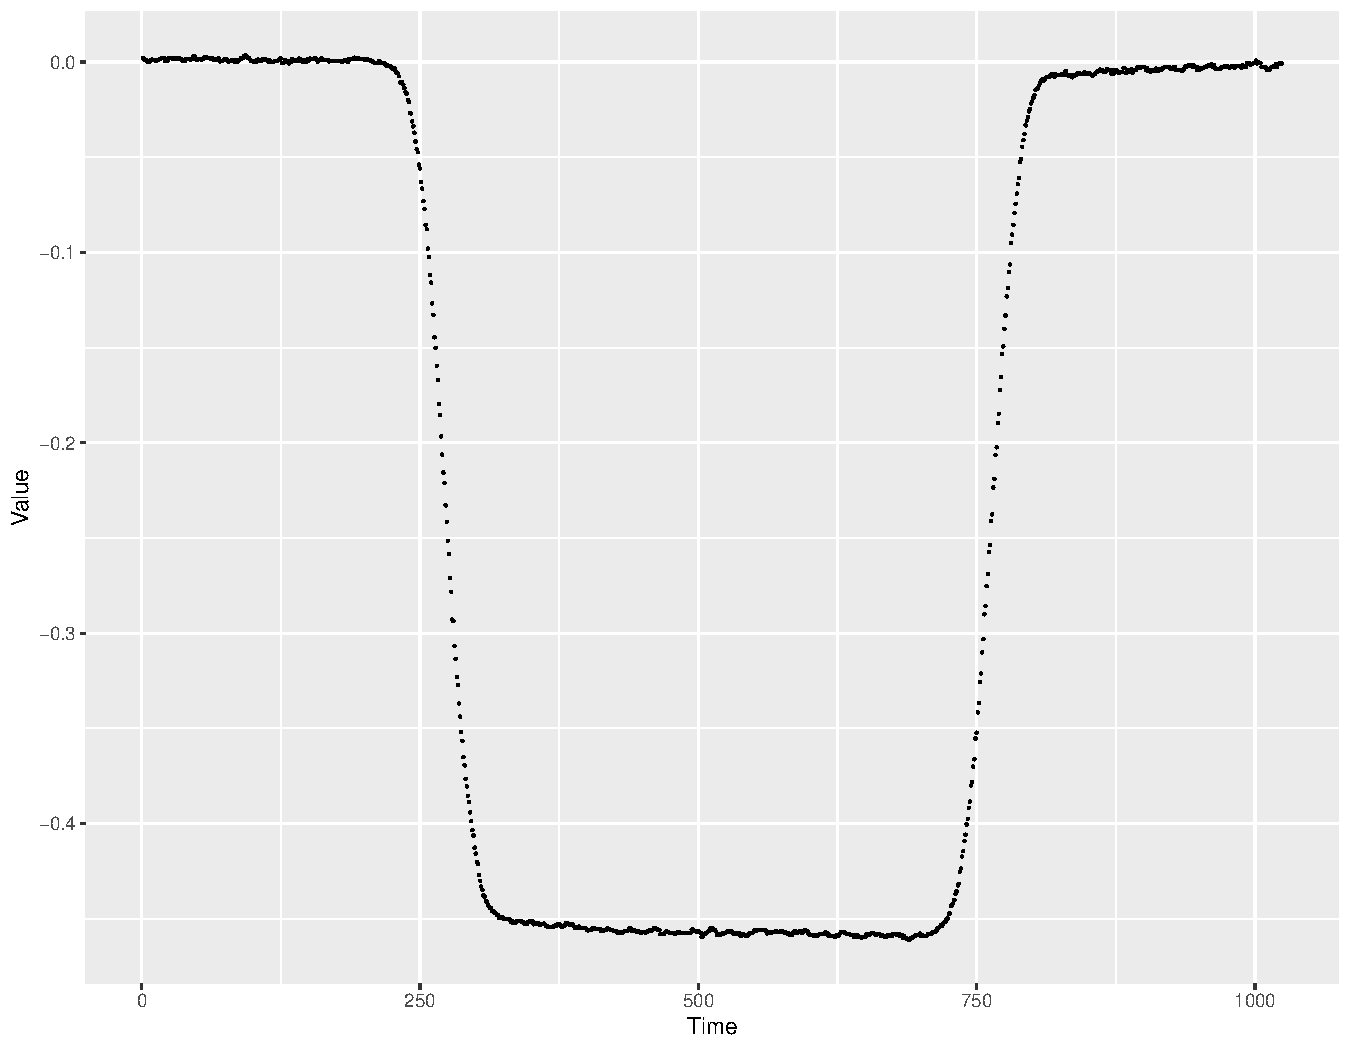
\includegraphics[width=\textwidth]{LabSrcs/resources/wave_smoothed_pic.pdf}
        \caption{Очищенный входной сигнал}
    \end{minipage}
\end{figure}
\begin{figure}[H]
    \centering
    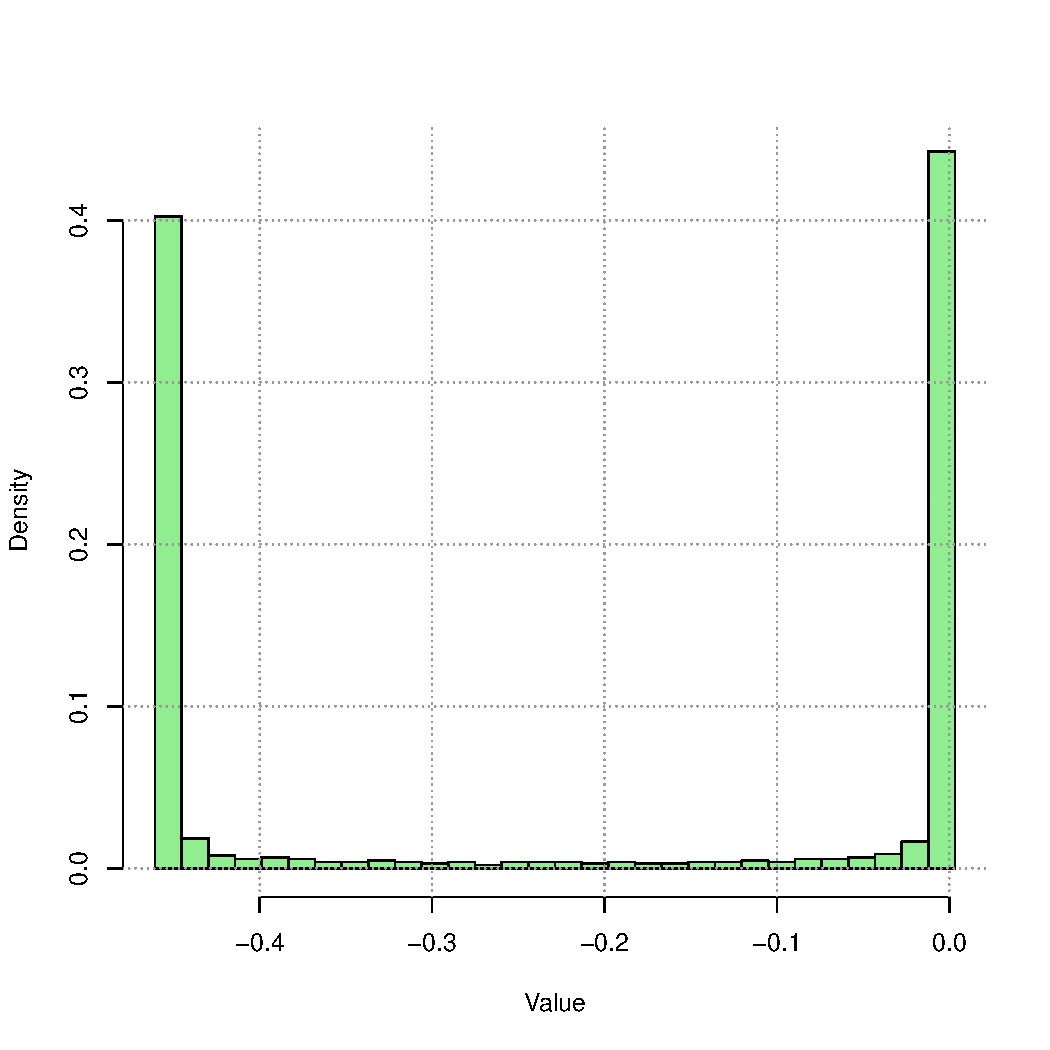
\includegraphics[width =0.7\textwidth]{LabSrcs/resources/wave_hist.pdf}
    \caption{Гистограмма сигнала}
    \label{fig:histsig}
\end{figure}
\begin{figure}[H]
    \centering
    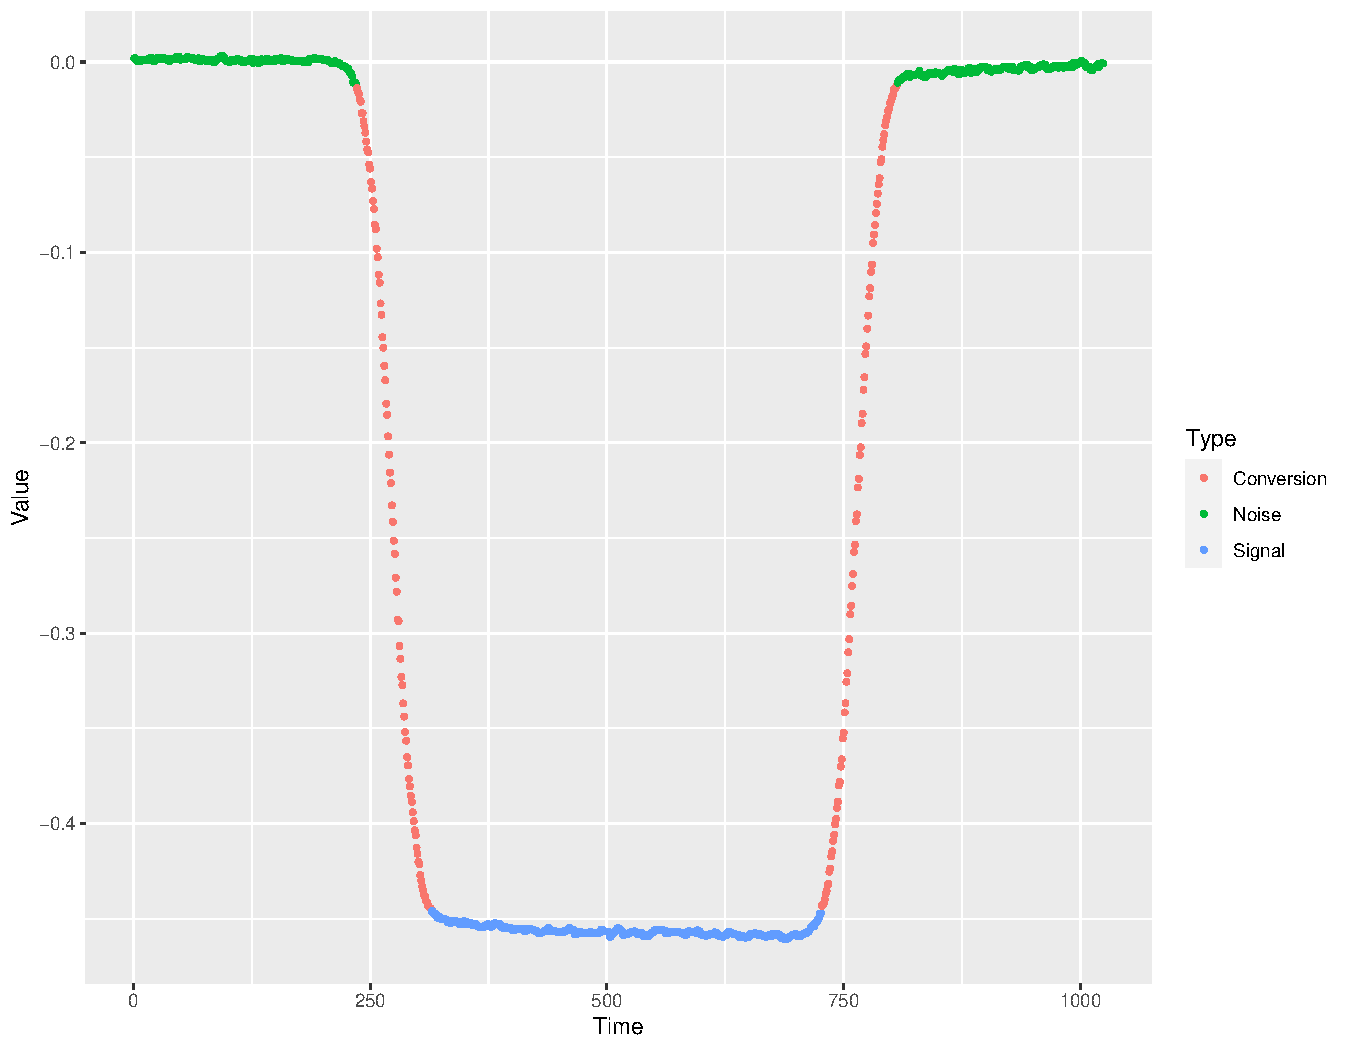
\includegraphics[width =0.9\textwidth]{LabSrcs/resources/wave_colored_pic.pdf}
    \caption{Разделение областей для очищенного сигнала}
    \label{fig:colwave}
\end{figure}
\begin{table}[H]
    \centering
    \begin{tabular}{|c|c|c|c|}
    \hline
         Промежуток&Тип&Количество разбиений&Критерий Фишера\\\hline 
1&Фон&8&0.99 \\\hline 
2&Переход&8&69.19 \\\hline 
3&Сигнал&8&1.88 \\\hline 
4&Переход&8&70.99 \\\hline 
5&Фон&8&3.69 \\\hline 

    \end{tabular}
    \caption{Характеристики выделенных областей}
    \label{tab:ftesttab}
\end{table}
\section{Обсуждение}
\subsection{Выборочные коэффициенты корреляции и эллипсы рассеивания}
\begin{itemize}
    \item \begin{enumerate}
    \item Для двумерного нормального распределения выполняется следующее соотношение:
    \begin{equation*}
        D(r)\leq D(r_S) \leq D(r_Q).
    \end{equation*}
    \item Для смеси нормальных распределений выполняется следующее соотношение:
    \begin{equation*}
        D(r_Q)< D(r_S)< D(r).
    \end{equation*}
\end{enumerate}
\item В каждом из экспериментов эллипс рассеивания покрывает не менее $95\%$ элементов выборки, то есть полученный результат согласуется с теоретическими ождианиями.  
\end{itemize}
\subsection{Оценки коэффициентов линейной регрессии}
На выборке без возмущений МНК дает более точные оценки коэффициентов линейной регрессии, чем МНМ. Однако МНМ более устойчив к редким выбросам и показывает лучшие, чем МНК, результаты на выборке с возмущениями.
\subsection{Метод хи-квадрат}
\begin{itemize}
    \item По результатам проверки на близость с помощью критерия $\chi^2$ гипотеза о нормальности двадцатиэлементной выборки, сгенерированной по закону $N(0,1)$, принята.
    \item Критерий, однако, также принял гипотезу о нормальности выборок, сгенерированных по законам $L(0,\frac{1}{\sqrt{2}})$ (Лапласа) и $U(-1.5,1.5)$ (равномерная). Таким образом, метод хи-квадрат нечувствителен на выборках малого размера.
\end{itemize}
\subsection{Дисперсионный анализ с применением критерия Фишера}
По результатам эксперимента можно сделать вывод, что наиболее однородными областями являются 1 фоновая область, сигнал, 2 фоновая область. Переходные области, для которых значение Фишера много больше 1, являются, таким образом, областями неоднородности.
\section*{Примечание}
С кодом работы и отчета можно ознакомиться по ссылке:\\\url{https://github.com/Kozlov992/MS_report5_6}\\
Код лабораторных находится в папке LabSrcs в файлах с расширением .pdf.
\begin{thebibliography}{9}
\bibitem{book1} 
 Вероятностные разделы математики. Учебник для бакалавров технических направлений.//Под ред. Максимова Ю.Д. $-$ Спб.: <<Иван Федоров>>, 2001. $-$ 592 c., илл.

\end{thebibliography}
\end{document}
